\documentclass[a4paper,11pt, twocolumn]{article}
\usepackage[margin=0.8in]{geometry}
\usepackage{xcolor}
\usepackage{graphicx} %package to manage images
\graphicspath{ {./images/} }
\usepackage{amssymb}

\title{AS-05 Operational Amplifiers}
\author{Revision sheet}
\date{}

\usepackage{fancyhdr}
\pagestyle{fancy}
\fancyhead{} % clear all header fields
\renewcommand{\headrulewidth}{0pt} % no line in header area
\fancyfoot{} % clear all footer fields
\renewcommand{\footrulewidth}{0.4pt}
\fancyfoot[C]{\thepage} % page number in centre of the page
\fancyfoot[R]{\footnotesize Thomas Boxall \\ Images from WJEC E-Book} % right hand footer has author name on top line and images reference on bottom line
\fancyfoot[L]{\footnotesize AS-05 Operational Amplifiers \\ Revision sheet} % left hand footer has title of document on top line and 'Revision Sheet' on bottom line


\begin{document}

\maketitle
\thispagestyle{fancy}

% CONTENTS OF THE REVISION SHEET HERE
\section{Introduction To Amplifiers}
Amplifiers take an analogue signal as an input, multiply it by the \textit{gain} then output the value.
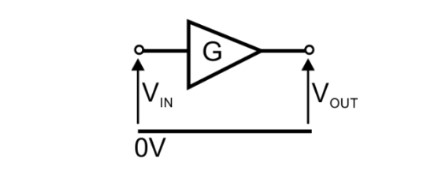
\includegraphics[width=0.45\textwidth]{basicAmp.jpg}
Voltage gain ($G$) can be calculated using the following equation.\\
$\displaystyle G = \frac{V_{OUT}}{V_{IN}}$\\
There are two broad categories of amplifer - non inverting which just amplifies the signal and inverting which amplifies the signal and inverts it.

\section{Op Amp}
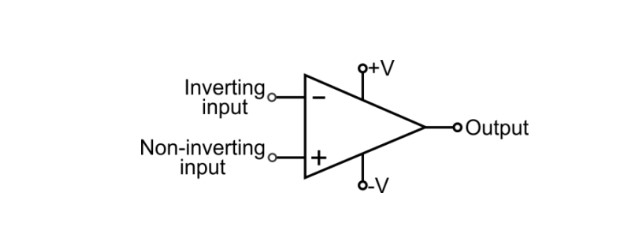
\includegraphics[width=0.45\textwidth]{opAmp.jpg}\\
Op-Amps have two inputs, inverting and non inverting. They require dual rail supply (positive and negative), these are usually not shown in circuit diagrams however. It amplifies the difference between the two input voltages. 
\subsection{Feedback}
This is where you feed some of the output back into the input. There are two types.
\subsubsection{Positive Feedback}
A portion of the output signal is fed back into the amplifer input. This causes the output signal to grow uncontrollably, which is bad.
\subsubsection{Negative Feedback}
This is where a portion of the output signal is subtracted from the input. It can be used to set the gain and reduce the distortion of the amp. The gain of the amplifier depends only on the feedback fraction.
\subsection{Saturation}
Op-Amps have a value at which they saturate. They cannot produce voltages above this point. When this happens, they distort the signal, in the method of clipping distortion.\\
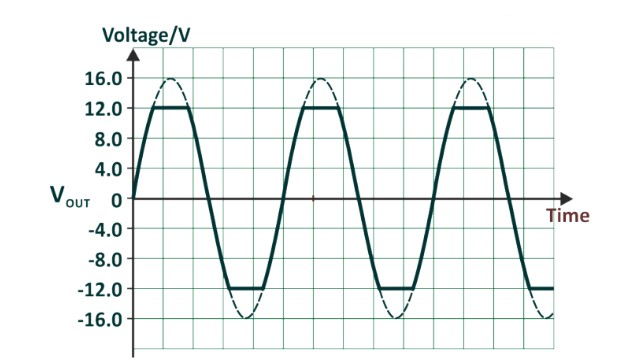
\includegraphics[width=0.45\textwidth]{clippingDistortion.jpg}

\section{Inverting Amplifier}
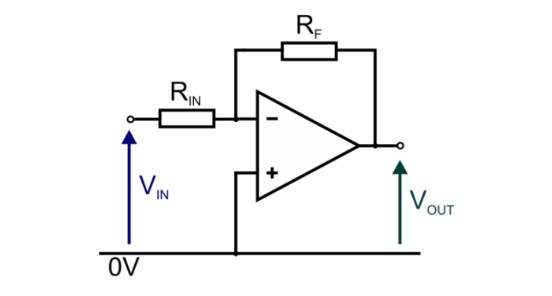
\includegraphics[width=0.45\textwidth]{invertingAmp.jpg}\\
$\displaystyle G= \frac{-R_F}{R_{IN}}$
\subsection{Input Impedance}
The input impedance of an inverting amplifier is $R_{IN}$. 
\subsection{Example}
In this example, the top graph shows the input voltage which has peak value of 2V. This 2V is multiplied by the gain of -3 to produce $\pm$6V. The waveform is inverted whilst the time period and frequency remain unchanged.
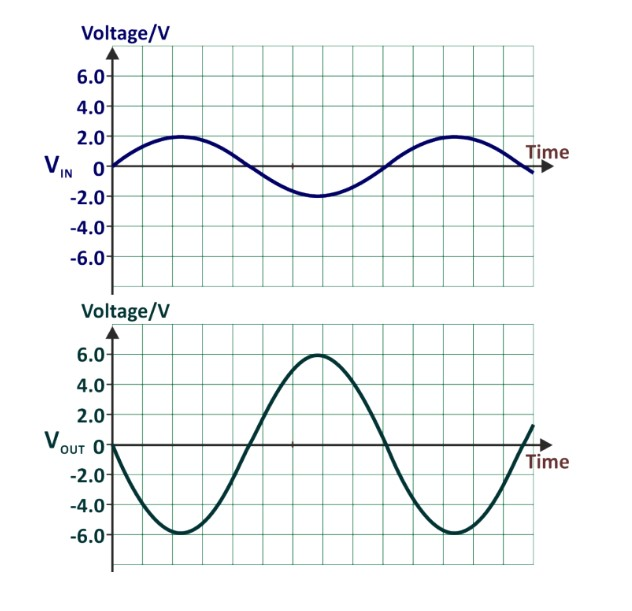
\includegraphics[width=0.45\textwidth]{invAmp-1.jpg}
\subsection{Saturation}
The op-amp saturates at $\pm$12V. This can be seen on the following graph.
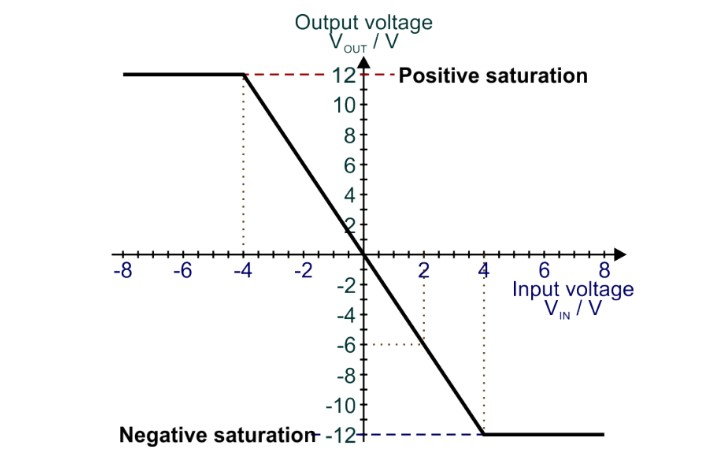
\includegraphics[width=0.45\textwidth]{invAmp-2.jpg}

\section{Non-Inverting Amplifier}
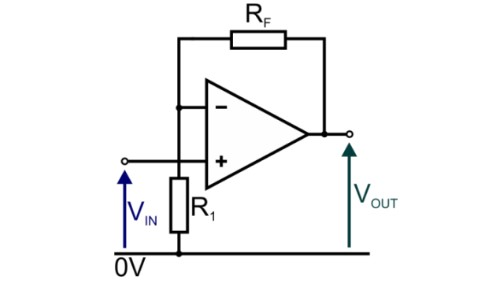
\includegraphics[width=0.45\textwidth]{nonAmp.jpg}\\
$\displaystyle G = 1+ \frac{R_F}{R_{IN}}$
\subsection{Input Impedance}
The input impedance of a non-inverting amplifier is the input impedance of the op-amp it is built from. 
\subsection{Example}
In this example, the top graph shows the input voltage which has a peak value of 1V. This 1V is multiplied by the gain of 4 to produce $\pm$4V. The waveform, time period and frequency are unchanged.
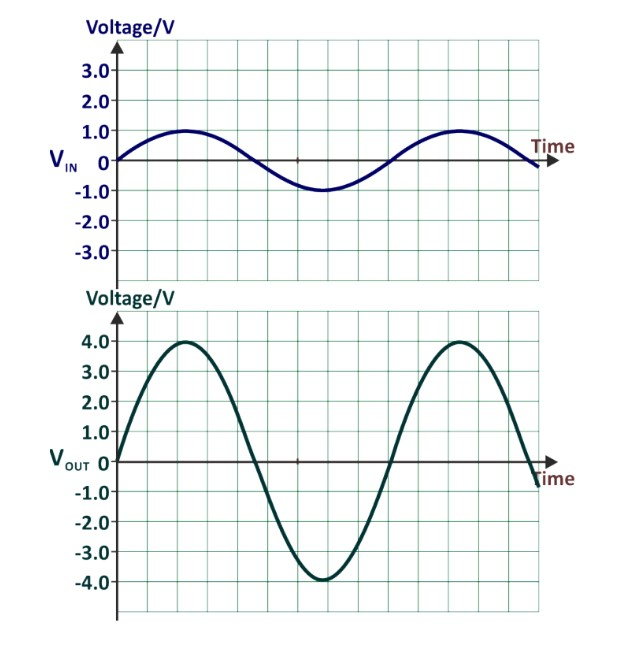
\includegraphics[width=0.45\textwidth]{nonAmp-1.jpg}
\subsection{Saturation}
The op-amp saturates at $\pm$10V. This can be seen on the graph below.
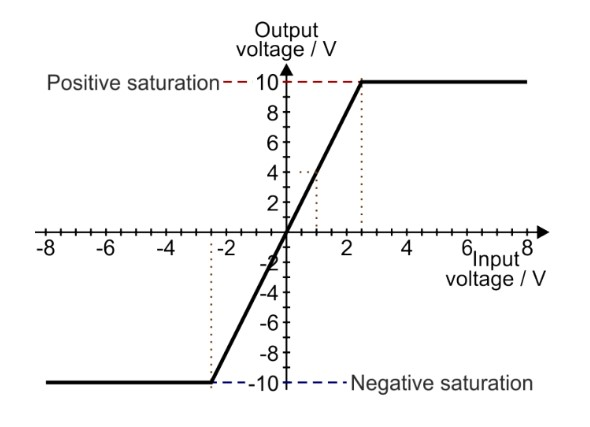
\includegraphics[width=0.45\textwidth]{nonAmp-2.jpg}

\section{Real World Op-Amps}
\subsection{Bandwidth}
Bandwidth is the range of frequencies that the amplifier can re-produce. It is shown on a graph called a frequency response graph.
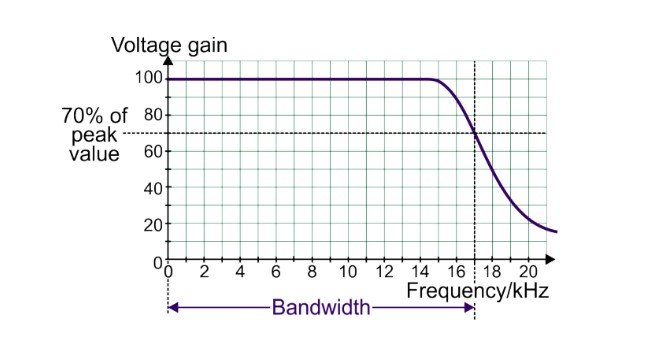
\includegraphics[width=0.45\textwidth]{freqResp.jpg}
Bandwidth is the point at which the gain drops to $\frac{1}{\sqrt{2}}$ (70\%) of its peak value. 
\subsection{GBP}
\textit{Gain Bandwidth Product} (GBP) is a property of the op-amp. It can be calculated using the following formula\\
$GBP = gain \times bandwidth$\\
It has the units $Hz$ and will usually be in the $MHz$. 
\subsection{CMRR}
\textit{Common Mode Rejection Ratio} (CMRR) is the ratio of the common-mode gain to differential-mode gain. Ideal op-amps should have infinite CMRR. Real op-amps have some CMRR, the higher it is the better it is. 
\subsection{Slew Rate}
Slew Rate specifies how quickly the output voltage can change in response to a change in input voltage. The higher the slew rate, the better as this means it takes a shorter time to change. Slew rate is specified on op-amp data sheets.
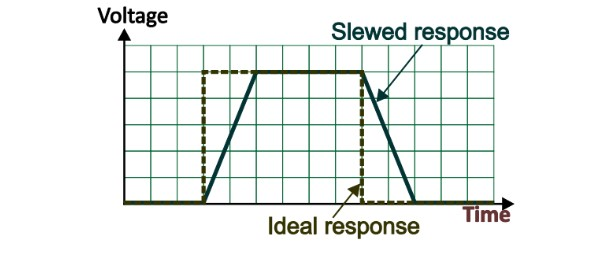
\includegraphics[width=0.45\textwidth]{slewRate.jpg}\\
Slew-Rate can be calculated by using the following formula.\\
$\displaystyle Slew\ Rate = \frac{\Delta V}{\Delta t}$
\subsection{Sine Waves}
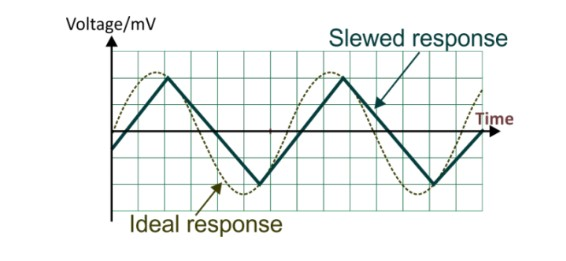
\includegraphics[width=0.45\textwidth]{slewRateSine.jpg}\\
When a sine wave gets distorted enough, it can become a triangular wave. To overcome this, we have to choose an op-amp with a high enough slew-rate to cope with our highest frequency signal. The following equation can be used to calculate the slew rate required for a distortion free output. \\
$\displaystyle Slew\ Rate = 2\pi f V_p$

\section{Summing Amplifier}
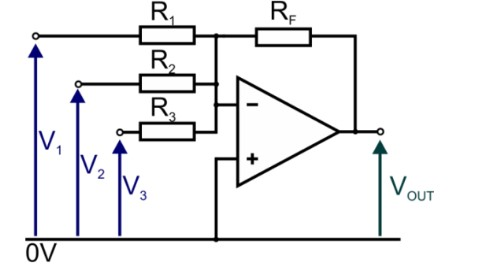
\includegraphics[width=0.45\textwidth]{summingAmp.jpg}
The Virtual Ground Summing Amplifier is used in digital to analogue counters and sound mixers. The value of $V_{OUT}$ can be calculated using the following equation:\\
$\displaystyle V_{OUT} = -R_{F} \left(\frac{V_1}{R_1}+ \frac{V_2}{R_2} + \frac{V_3}{R_3}+ \ldots \right)$\\
The equation can be expanded or shrunk to fit as many inputs as required. As this makes use of an inverting amplifier design, the output is inverted. This can be reversed by adding another standard inverting amplifer to the output, with $R_F$ and $R_1$ equal, so that no gain is applied, as seen in the diagram below.
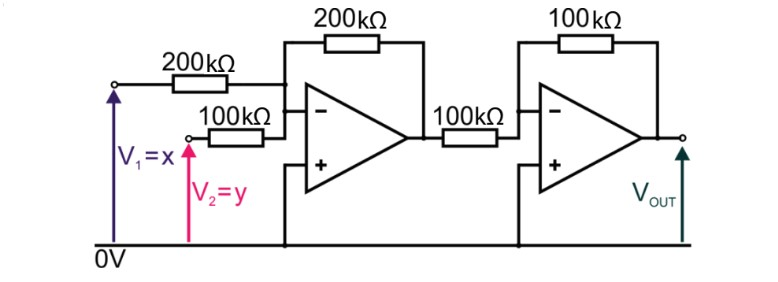
\includegraphics[width=0.45\textwidth]{summinigAmpInverted.jpg}

\section{Voltage Follower}
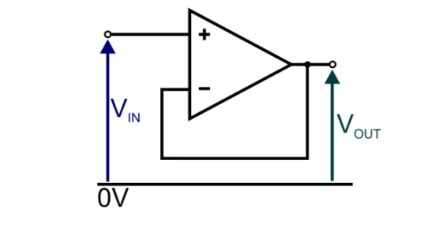
\includegraphics[width=0.45\textwidth]{voltageFollower.jpg}\\
This can be used as an impedance buffer. It can reduce the resistance so that a subsystem connected after the buffer gets the right resistance and current. 

\section{Comparator}
This compares the input and outputs a value depending on which is bigger. \\
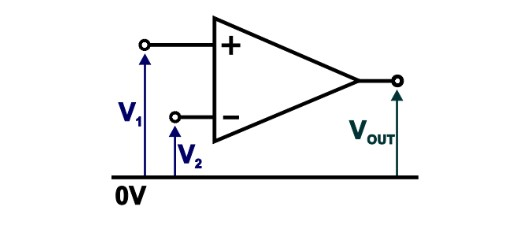
\includegraphics[width=0.45\textwidth]{comparator.jpg}\\
If $V_+>V_- \therefore V_{OUT} = +V_{sat}$\\
If $V_->V_+ \therefore V_{OUT} = -V_{sat}$\\
We can set $V_-$ to a fixed value then the comparator will tell us if $V_+$ is bigger or smaller. A photodiode could be used as part of the sensor subsystem. 



\end{document}


Introduction
op amp
    feedback (pos and neg)
inverting
    input impedance
non inverting
    input impedance
Real World
    bandwidth
    gbp
    cmrr
    slew rate
summing Amplifiers
    with non inverted output
voltage follower/buffer
comparators
photodiode?
clipping distortion & others?